%%%%%%%%%%%%%%%%%%%%%%%%%%%%%%%%%%%%%%%%%
% Short Sectioned Assignment
% LaTeX Template
% Version 1.0 (5/5/12)
%
% This template has been downloaded from:
% http://www.LaTeXTemplates.com
%
% Original author:
% Frits Wenneker (http://www.howtotex.com)
%
% License:
% CC BY-NC-SA 3.0 (http://creativecommons.org/licenses/by-nc-sa/3.0/)
%
%%%%%%%%%%%%%%%%%%%%%%%%%%%%%%%%%%%%%%%%%

%----------------------------------------------------------------------------------------
%	PACKAGES AND OTHER DOCUMENT CONFIGURATIONS
%----------------------------------------------------------------------------------------

\documentclass[paper=a4, fontsize=11pt]{scrartcl} % A4 paper and 11pt font size
\usepackage{graphicx}
\usepackage{hyperref}
\usepackage[T1]{fontenc} % Use 8-bit encoding that has 256 glyphs
\usepackage{fourier} % Use the Adobe Utopia font for the document - comment this line to return to the LaTeX default
\usepackage[english]{babel} % English language/hyphenation
\usepackage{amsmath,amsfonts,amsthm} % Math packages

\usepackage{lipsum} % Used for inserting dummy 'Lorem ipsum' text into the template

\usepackage{sectsty} % Allows customizing section commands
\allsectionsfont{\centering \normalfont\scshape} % Make all sections centered, the default font and small caps

\usepackage{fancyhdr} % Custom headers and footers
\pagestyle{fancyplain} % Makes all pages in the document conform to the custom headers and footers
\fancyhead{} % No page header - if you want one, create it in the same way as the footers below
\fancyfoot[L]{} % Empty left footer
\fancyfoot[C]{} % Empty center footer
\fancyfoot[R]{\thepage} % Page numbering for right footer
\renewcommand{\headrulewidth}{0pt} % Remove header underlines
\renewcommand{\footrulewidth}{0pt} % Remove footer underlines
\setlength{\headheight}{13.6pt} % Customize the height of the header

\numberwithin{equation}{section} % Number equations within sections (i.e. 1.1, 1.2, 2.1, 2.2 instead of 1, 2, 3, 4)
\numberwithin{figure}{section} % Number figures within sections (i.e. 1.1, 1.2, 2.1, 2.2 instead of 1, 2, 3, 4)
\numberwithin{table}{section} % Number tables within sections (i.e. 1.1, 1.2, 2.1, 2.2 instead of 1, 2, 3, 4)

\setlength\parindent{0pt} % Removes all indentation from paragraphs - comment this line for an assignment with lots of text

%----------------------------------------------------------------------------------------
%	TITLE SECTION
%----------------------------------------------------------------------------------------

\newcommand{\horrule}[1]{\rule{\linewidth}{#1}} % Create horizontal rule command with 1 argument of height

\title{	
\normalfont \normalsize 
\textsc{University of Amsterdam} \\ [25pt] % Your university, school and/or department name(s)
\horrule{0.5pt} \\[0.4cm] % Thin top horizontal rule
\huge Movement of Ants \\ % The assignment title
\horrule{2pt} \\[0.5cm] % Thick bottom horizontal rule
}

\author{Georgios Methenitis} % Your name

\date{\normalsize\today} % Today's date or a custom date

\begin{document}

\maketitle % Print the title

%----------------------------------------------------------------------------------------
%	PROBLEM 1
%----------------------------------------------------------------------------------------
\section*{Abstract}
In this paper, a foraging algorithm is presented, which simulates the movement of ants in a two dimensional space. Section~\ref{intro}, serves an introduction to this paper, Section~\ref{related} includes some related work that we based on, and Section~\ref{approach}, presents the actual approach that we follow. In Section~\ref{results}, experiments and results are presented, Section~\ref{future}, talks about some future work that can be done in our work, and finally, Section~\ref{conclusion}, concludes this paper.

\section{Introduction}
\label{intro}
Ants are social insects of the family Formicidae. Big ants' average speed is 300 meters per hour, which considered to be really fast, knowing that if humans had the same size as ants, we would have been able to achieve speeds less than 20 meters per hour. Foraging ants travel distances of up to 200 meters from their nest. But the actual reason that ants show this complicated social behavior is the fact that they can communicate with each other using pheromones, sounds, and touch.

\section{Related Work}
\label{related}
\cite{1}~This paper presents a box simulator for ants, software that allows the simulation of ants in a restricted environment. They demonstrate how some parameters affect their performance on finding a solution to a given problem. They also use a model for exploring as ants are not walking randomly in the two dimensional space, but knowing their previous move they choose their next move from a Gaussian distribution, leading to a more natural exploring procedure.

\cite{2}~Ants present a very good natural metaphor to evolutionary 
computation. While their individual computational power is small 
compared to more evolved species, it is the power of their colonies 
that inspire computer scientists. This paper presents ``Ants Box 
Simulator'', software that allows the simulation of ants in a restricted 
environment. They demonstrate how some parameters affect their 
performance on finding a solution to a given problem. They use two kinds of pheromone to solve the problem, one kind to lead ants to their nest and to the food source.

\section{Approach}
\label{approach}
In this section, our approach is going to be presented. First, some important details of the approach are presented. Later in this section, we are looking deep into the algorithm's functions for different purposes.

Box simulator, as we saw in the related work, both related simulation were using this box simulator approach, in this work we use the same two dimensional approach to simulate a small portion of the real environment, with constraints such as that the space is missing a dimension and also that the size is fixed. Although, we use a huge space $500 \times 500$, which has $250.000$ cells.

Moreover, in this space, we have fixed points in two dimensional space to represent the nest and the food source. Obstacles can also be added in the simulation, ants cannot walk through obstacles and we use them to experiment with the algorithm's behavior when more constraints take part into the simulation.

As in~\cite{2}, we use two kinds of pheromone. A pheromone connected to the ants' ability to find food, and another kind of pheromone which is related with their navigation back to their nest.

As it is described in both related works, and it is been followed in this, ants are independent agents with no ability to ``speak'' to each other but only following the right pheromone, in order to have exploitative agents we use, $\epsilon$-greedy approach. Ants can do $9$ different movements to all the neighboring cells including their own cell.

Diffusion and evaporation are also used because these two are natural phenomena that happen in the ants' environment. We include this two functions to have a more realistic simulation, although the parameter tuning for these two function was tough, as there is no information in the literature for these phenomena.


\subsection{Simulation}
When the simulation starts, all ants are located at their nest. Ants also have a hunger level, which is equal to the maximum value, $h = 1.0$, $h \in [0.0,1.0]$, meaning that ants are eager to find food. Because of no exploration all the values of food pheromone are $0.0$, resulting to a random walk by the ants. While they are exploring, they are dropping home pheromone as they are located in their nest:
\begin{equation}
{ph\_{home}}_t^{i,j} = max\_ph\_home, if\ i,j = nest
\end{equation}
When they move out of their nest they leave trails of home pheromone:
\begin{equation}
{ph\_{home}}_t^{i,j} = ||{ph\_{home}}_{t-1}^{i,j} - \beta||
\end{equation}
Eventually, some ants will find the food source. When this happens, ants are dropping a maximum value of food pheromone in the cell that they found the food:
\begin{equation}
{ph\_{food}}_t^{i,j} = max\_ph\_food, if\ i,j = food
\end{equation}
Ants leave trails also in the case of food pheromone as they move out from the food source following the same equation~(3.2).
When the ants have $h < hunger\_threshold$, $0.3$ is used. They want to go back at their nest. But when the ants have $h \geq hunger\_threshold$, they want to go find food again.

\subsection{Epsilon-greedy}
Epsilon-greedy action selection is used by all the agents. The best action is selected for a proportion $1 - \epsilon$ of the trials, and another action is randomly selected for a proportion $\epsilon$. A typical parameter that is used is: $\epsilon = 0.2$, but this can vary. Depending where they want to go, they follow with $\epsilon$-greedy the pheromone. When greedy action is chosen, ants select the cell with the maximum pheromone.


\subsection{Diffusion and Evaporation}
Two important functions in the simulation are diffusion and evaporation, the next two equations are describing these features of the simulation. First equation is describing diffusion. The amount of pheromone in timestep $t$ in one cell is the maximum between the previous amount of pheromone in the same cell and the maximum scaled value of all the neighboring cells.
\begin{equation}
{ph}_t^{i,j} = max[{ph}_{t-1}^{i,j}, r_d * \smash{\displaystyle\max_{-1 \leq x,y \leq 1}}[{ph}_{t-1}^{i+x,j+y}], x,y \in \mathbb{R}
\end{equation}
$r_d \in [0.0,1.0]$, diffusion rate.\\

For evaporation things are simpler. The amount of pheromone in timestep $t$ in one cell is the scaled value of the same cell in the previous step $t-1$. 
\begin{equation}
{ph}_t^{i,j} = r_e * {ph}_{t-1}^{i,j}
\end{equation}
$r_e \in [0.0,1.0]$, evaporation rate.\\

\section{Results}
\label{results}
Apart from the simulation algorithm we also focused on making an appropriate graphical user interphase to visualize the all the simulation details. Figure~\ref{fig1}, illustrates the gui that is made for this purpose. 
The screen in the middle is the actual ants' environment, the left hand side screen is responsible to render how much have the ants explored the world. Last, the two screens on the right depict the home and the food pheromone in each cell, with white gradient to visualize the amount of it. In this interphase you can start, pause and reset the simulation. The number of ants and the speed of the simulation can also be changed. Rendering functions can also be enabled or disabled, for ants, pheromone and exploration. We can also show the average value of hunger among the ants' society.

\begin{figure}[h!]
  \caption{Graphical user interphase.}
  \label{fig1}
  \centering
    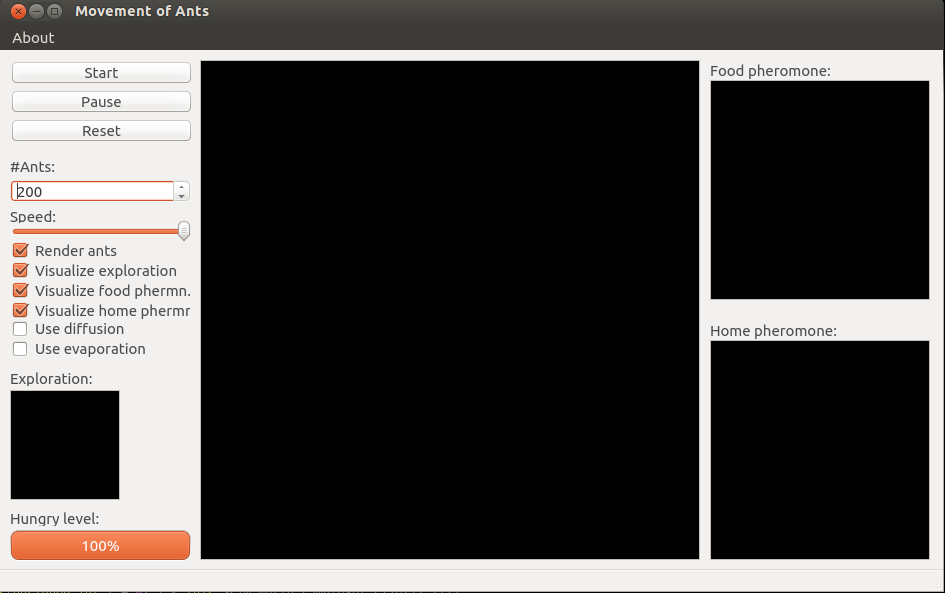
\includegraphics[width=0.7\textwidth]{gui.png}
\end{figure}

Figures~\ref{fig2} and~\ref{fig3}, illustrate the results of the simulation when it converges to a permanent solution, which is optimal but only considering the Manhattan distance. One thing that lead to this strange behavior is that we count diagonal moves the same as all the straight moves, so ants they can do a diagonal move that ``costs'' the same as a normal move. Although, the pheromone updates as well as the diffusion, take into account the actual distance between two pixels. So, diagonal updates, update the pheromone with distance $\sqrt{2}$, and that is the reason, we see no geometrically optimal solution.

\begin{figure}[h!]
  \caption{Experiment without obstacle.}
  \label{fig2}
  \centering
    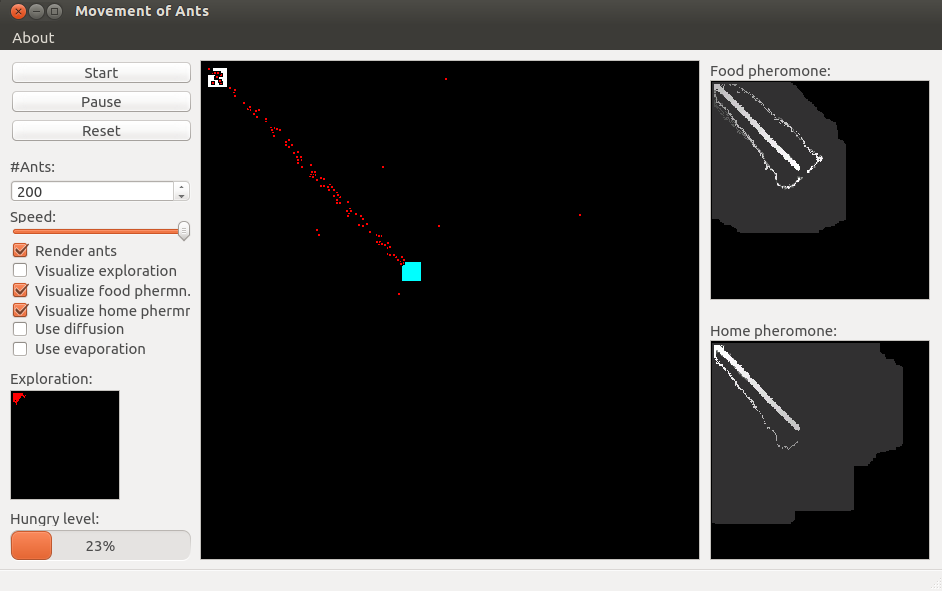
\includegraphics[width=0.7\textwidth]{noObstacle.png}
\end{figure}

\begin{figure}[h!]
  \caption{Experiment with obstacle.}
  \label{fig3}
  \centering
    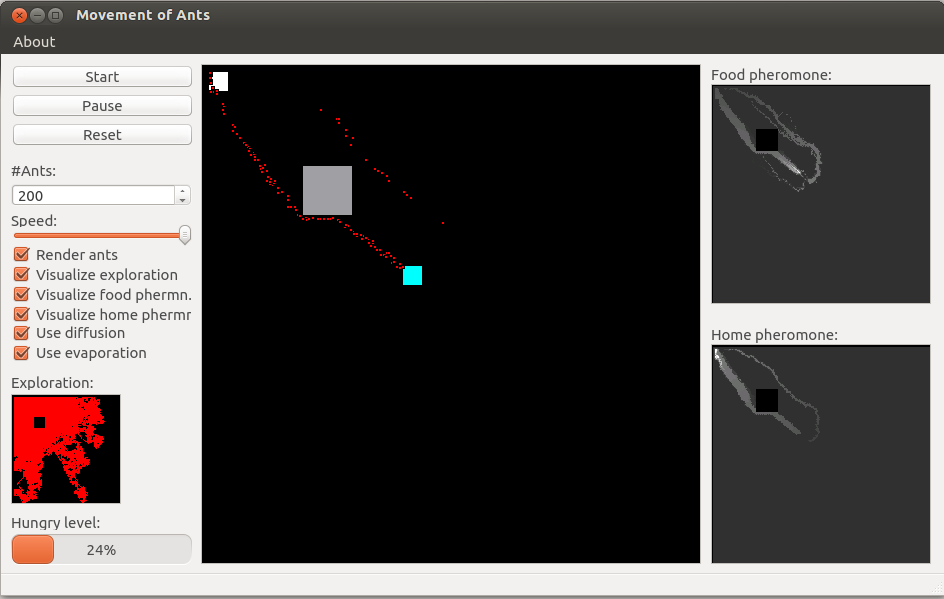
\includegraphics[width=0.7\textwidth]{obstacle.png}
\end{figure}

\section{Future Work}
\label{future}
Even though that the simulation converges to a Manhattan optimal solution, some constant variables need to be reconsidered, as it is really tough to be estimated. Furthermore, one thing that could be included are the birth and the death rates of the ants, so we are going to have multiple generations of them. A logistic growth model can be used for this purpose, with carrying capacity to put an upper bound to the population.


\section{Conclusion}
\label{conclusion}
In this paper we have presented a software with a graphical interphase which simulates and visualizes the behavior of ants.

\newpage
\begin{thebibliography}{9}

\bibitem{1}
  Liviu A. Panait and Sean Luke,
  \emph{Ant Foraging Revisited}.
  George Mason University, Fairfax, VA 22030
\bibitem{2}
Paulo E. Merloti 
\emph{Simulation of Artificial Ant's Behavior 
in a Digital Environment}.
Department of Computer Science 
Graduate Seminar in Artificial Intelligence 
Evolutionary and Adaptive Computation
\bibitem{p2}\href{http://www.ehow.com/about_5365350_fast-can-ant-run.html}{How Fast Can an Ant Run?}
\bibitem{p2}\href{http://en.wikipedia.org/wiki/Ant}{Wiki: Ant}
\bibitem{p2}\href{http://en.wikipedia.org/wiki/Ant_colony_optimization_algorithms}{Ant colony optimization algorithms}
  

  \end{thebibliography}

\end{document}